\section{Decorated Teichm\"uller theory}

First we review some background on decorated Teichm\"{u}ller spaces. For a detailed reference, see~\cite{penner_12}.
%
Let $S$ be a surface with boundary, and let $p_1,\dots,p_n$ be a collection of marked points on the boundary,
such that each boundary component contains at least one marked point. More generally, we can also have a collection of interior marked points (or \emph{punctures}),
but we will not be concerned with this case in this paper. We also equip the surface with a triangulation, where the arcs terminate
at the marked boundary points. The \emph{Teichm\"{u}ller space} of~$S$, denoted~$\mathcal{T}(S)$, is the space of (equivalence classes of) hyperbolic metrics on $S$ with constant negative
curvature, with cusps at the marked points. Because of the cusps, any geodesic between marked points has infinite hyperbolic length.

The \emph{decorated Teichm\"{u}ller space} of $S$, written $\widetilde{\mathcal{T}}(S)$, is a trivial vector bundle over $\mathcal{T}(S)$,
with fiber ${\mathbb R}_{> 0}^n$. The fibers represent a choice of a positive real number associated to each marked point.
At each marked point, we draw a horocycle whose size (or \emph{height}) is determined by the corresponding positive number.
Truncating the geodesics using these horocycles, it now makes sense to talk about their lengths. If $\ell$ is the truncated
length of one of these geodesic segments, then the $\lambda$-length (or \emph{Penner coordinate}) associated to that geodesic arc
is defined to be
\[ \lambda := \exp(\ell/2). \]

Fixing a triangulation of the marked surface, the collection of $\lambda$-lengths corresponding to the arcs in the triangulation (including segments
of the boundary) form a system of coordinates for~$\widetilde{\mathcal{T}}(S)$. Choosing a different triangulation results in a different
system of coordinates, but they are related by simple transformations which are a hyperbolic analogue of Ptolemy's theorem from classical Euclidean geometry.
If two triangulations differ by the flip of a single arc as in Figure~\ref{fig:ptolemy},
then the $\lambda$-lengths are related by $ef = ac + bd$.

\input{flip.tex}

\section[Laurent expression for lambda-lengths]{Laurent expression for $\boldsymbol{\lambda}$-lengths}

In this paper, we will only be concerned with the case that the surface $S$ is a disk with marked points on its boundary (which we will
picture as a convex polygon). So we restrict to that case now.

Fix a triangulation of an $n$-gon, and label the vertices $1$ through $n$.
Schiffler~\cite{schiffler_08} defined a~\emph{$T$-path} from $i$ to $j$ to be a sequence
\[ \alpha = \big(a_0,\dots,a_{\ell(\alpha)} \,|\, t_1,\dots,t_{\ell(\alpha)}\big) \]
such that
\begin{itemize}\itemsep=0pt
 \item[(T1)] $a_0,\dots,a_{\ell(\alpha)}$ are vertices of the polygon,
 \item[(T2)] $t_k$ is an arc in the triangulation connecting $a_{k-1}$ to $a_k$,
 \item[(T3)] no arc is used more than once,
 \item[(T4)] $\ell(\alpha)$ is odd,
 \item[(T5)] if $k$ is even, then $t_k$ crosses the arc connecting vertices $i$ and $j$,
 \item[(T6)] if $k < l$ and both $t_k$ and $t_l$ cross the arc from $i$ to $j$, then
 the point of intersection with $t_k$ is closer to $i$, and the point of intersection
 with $t_l$ is closer to $j$.
\end{itemize}

An example of a $T$-path in a hexagon is shown in Figure~\ref{fig:t_path}.
The even-numbered edges are colored blue, and the odd edges red, for emphasis.

\begin{figure}[h!] \centering

 \begin {tikzpicture}[scale=1.3]
 \coordinate (A) at (-1,0);
 \coordinate (B) at (-0.5,-0.866);
 \coordinate (C) at (0.5,-0.866);
 \coordinate (D) at (1,0);
 \coordinate (E) at (0.5,0.866);
 \coordinate (F) at (-0.5,0.866);

 \draw (A) -- (B) -- (C) -- (D) -- (E) -- (F) -- cycle;

 \draw (B) -- (F) -- (C) -- (E);

 \draw (A) node[left] {$i$};
 \draw (D) node[right] {$j$};

 \draw[red, line width = 1.2] (A) -- (B);
 \draw[red, line width = 1.2] (F) -- (E);
 \draw[red, line width = 1.2] (C) -- (D);

 \draw[blue, line width = 1.2] (B) -- (F);
 \draw[blue, line width = 1.2] (E) -- (C);
 \end {tikzpicture}

 \caption{A $T$-path from $i$ to $j$.} \label {fig:t_path}
\end{figure}

We denote the set of all $T$-paths from $i$ to $j$ by $T_{ij}$. Given a $T$-path $\alpha$,
we define a Laurent monomial $x_\alpha$ (in terms of the $\lambda$-lengths of a fixed triangulation) as
the product of the $\lambda$-lengths used in the $T$-path, with the even-numbered ones inverted. That is,
if the ordered sequence of edges in $\alpha$ is $e_1, e_2, \dots, e_{2m+1}$, then
\[ x_\alpha := \frac{\prod_{k=0}^m x_{e_{2k+1}}}{\prod_{k=1}^m x_{e_{2k}}}. \]

Schiffler proved the following theorem relating $\lambda$-lengths and $T$-paths.

\begin{Theorem}[{\cite[Theorem 1.2]{schiffler_08}}] Let $x_{ij}$ be the $\lambda$-length corresponding to the geodesic arc
 connecting vertices $i$ and $j$ in a triangulated polygon. Then
 \[ x_{ij} = \sum_{\alpha \in T_{ij}} x_\alpha. \]
\end{Theorem}

\begin{Remark} \label{rem:subtriang}\rm
As a consequence of the definition of $T$-paths, to compute $x_{ij}$ it is sufficient to consider only the sub-polygon consisting of the
triangles which the geodesic arc connecting vertices $i$ and $j$ crosses.
\end{Remark}

\section{Decorated super-Teichm\"{u}ller theory}\label{sec:dec_super}

Super-Teichm\"{u}ller spaces have been studied for several years now (see for example~\cite{cr_88}).
Recently, Penner and Zeitlin introduced a decorated version of super-Teichm\"{u}ller spaces~\cite{pz_19}.
It is generated by even variables corresponding to the
$\lambda$-lengths of a triangulation, as well as odd variables (called \emph{$\mu$-invariants}) corresponding to the triangles. They give
a super version of the Ptolemy relation, which reads as follows (see Figure~\ref{fig:super_ptolemy} for the meanings of the variables)
\begin{gather*}
 ef = (ac+bd)\left( 1+{{\sigma\theta\sqrt{\chi}}\over{1+\chi}}\right),\qquad
 \sigma' = {{\sigma-\sqrt{\chi}\theta}\over{\sqrt{1+\chi}}},\qquad
 \theta' = {{\theta+\sqrt{\chi}\sigma}\over{\sqrt{1+\chi}}},
\end{gather*}
where $ \chi = \frac{ac}{bd}$.

\input{superflip.tex}

We will usually find it convenient to re-write these equations without $\chi$, as follows
\begin{gather}
 ef = ac+bd+\sqrt{abcd} \sigma\theta, \label{eq:mutation}\\
 \sigma' = {{\sigma\sqrt{bd}-\theta\sqrt{ac}}\over{\sqrt{ac+bd}}}, \label{eq:mu_mutation_neg} \\
 \theta' = {{ \theta\sqrt{bd}+\sigma \sqrt{ac}}\over{\sqrt{ac+bd}}}.\label{eq:mu_mutation_pos}
\end{gather}
An important corollary of these equations is the following
\begin{equation}\label{eq:mu_cross}
	\sigma\theta=\sigma'\theta',
\end{equation}
which will be used frequently in our proofs.

To understand the oriented arrows in Figure~\ref{fig:super_ptolemy} and the minus sign in equation~\eqref{eq:mu_mutation_neg},
we need the combinatorial data of a \emph{spin structure}. In~\cite{cr_07} and~\cite{cr_08}, an isomorphism was shown between
the set of equivalence classes of spin structures on a surface and the set of isomorphism classes of Kasteleyn orientations
of a~fatgraph spine of the surface. Dual to any fatgraph spine is a~triangulation of the surface, and so an orientation of
the fatgraph corresponds to an orientation of a~triangulation (requiring the dual edge to cross from left to right). For our
purposes a~\emph{spin structure} will be a~choice of orientation of the edges of a~triangulation, modulo a~certain equivalence relation,
which we now describe.

Fix a triangulation $\Delta$ and an orientation $\tau$ of the edges in that triangulation. For any triangle~$t$,
consider the transformation which reverses the orientation of the three sides of~$t$. Define an equivalence relation on orientations by declaring that $\tau \sim \tau'$ if they differ by a~sequence of these transformations. In~\cite{pz_19}, a spin
structure is represented combinatorially by an equivalence class of orientations.

In \cite{pz_19}, the authors did not consider surfaces with boundary, as we do here. Because the orientation of boundary segments
will play no role in our formulas for $\lambda$-lengths (but not $\mu$-invariants), we can often ignore the boundary orientations.
Note that the hypothesis of Proposition~\ref{prop:equiv_rel} on the triangulation is sufficient because of Remark~\ref{rem:subtriang}.

\begin {Proposition} \label{prop:equiv_rel}
 Fix a triangulation of a polygon in which every triangle has at least one boundary edge. Then there is a unique spin structure after ignoring the boundary edges. In particular, this means that, from any representative orientation of a fixed spin structure, one can obtain all other orientations on the interior diagonals, without leaving this spin structure.
\end {Proposition}
\begin {proof}
 Because every triangle has at least one boundary edge, one can naturally sequence the triangles (and internal diagonals) from left-to-right.
 We may picture the polygon as follows, to emphasize this:
 \begin{center}
 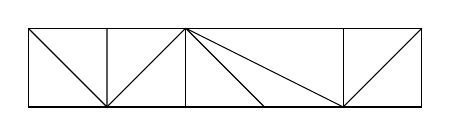
\begin{tikzpicture}
 \draw (0,0) -- (0,1) -- (5,1) -- (5,0) -- cycle;

 \draw (0,1) -- (1,0) -- (1,1);
 \draw (1,0) -- (2,1);

 \draw (2,1) -- (2,0);
 \draw (2,1) -- (3,0);
 \draw (2,1) -- (4,0);

 \draw (4,0) -- (4,1);
 \draw (4,0) -- (5,1);
 \end{tikzpicture}
 \end{center}
 We will demonstrate that we may change the orientation of a single edge while remaining in the same equivalence class. Label
 the triangles from left to right as $t_1,t_2,\dots$ and the internal diagonals as $d_1,d_2,\dots$. We will argue that we can change
 the orientation of just $d_k$, by induction on $k$.

 If $k=1$, then $d_1$ is an edge of $t_1$, and the other two edges of $t_1$ are on the boundary. Because we ignore boundary orientations,
 the equivalence relation allows us to reverse the orientation of just $d_1$.

 Now, for arbitrary $d_k$, reverse the orientations around triangle~$t_k$. This affects both $d_k$ and~$d_{k-1}$. But by induction, we may
 change just $d_{k-1}$ while staying in the equivalence class. This proves the claim.
\end {proof}

In Figure~\ref{fig:super_ptolemy}, the arrows on the edges labelled $e$ and $f$ represent the choice of orientation. In the figure,
the orientations of the edges around the boundary of the quadrilateral are not indicated. Three of the four edges are unchanged
in the super Ptolemy transformation, and only the orientation of the edge labelled~$b$ is changed, see Figure~\ref{fig:flip_spin}. The sign in equation~\eqref{eq:mu_mutation_neg} is determined by the relative positions of the triangular faces with respect to the chosen orientation.

\input{spin_flip.tex}

As illustrated in Figure~\ref{fig:flip_spin}, the super Ptolemy relation is \emph{not} an involution. Performing a flip
twice results in reversing the orientations around the top triangle. This leads us to the following observation that $\mu$-invariants are well-defined only up to sign. Consequently, in the main results of our paper regarding $\mu$-invariants (Theorems~\ref{thm:mu_single_fan} and~\ref{thm:proof_zigzag}), we must specify a mutation sequence to obtain a formula for the $\mu$-invariants.

\begin{Remark} \label{rem:mu-invariants}\rm
The above equivalence relation, i.e., as used in Proposition~\ref{prop:equiv_rel}, guarantees that the result after flipping twice represents the same spin structure, but algebraically it has the effect of negating the $\mu$-invariant of that triangle
($\theta \mapsto -\theta$ in the figure). This means that the specific $\mu$-invariants are not a feature of the triangulation
and spin structure alone, but also the choice of representative orientation. Choosing a different orientation corresponds to
changing the sign of some of the $\mu$-invariants.
\end{Remark}

\begin{Remark} \label{rem:lambda}\rm
Unlike the $\mu$-invariants, the expressions of $\lambda$-lengths in terms of an initial triangulation (as will be described more fully in Corollary~\ref{cor:laurent}) are independent of the orientation of the arc as part of a spin structure, and of the flip sequence used to obtain a triangulation containing that arc. This is proven in \cite{pz_19} in the case of surfaces without boundaries. The fact that $\lambda$-lengths are well-defined can also be seen as a consequence of the well-definedness of super-freizes, as we will describe in Sections~\ref{sec:super-friezes} and~\ref{sec:subfrieze}, based on \cite{M-GOT15,pz_19}. We provide a more direct proof in Appendix~\ref{appendix}.
\end{Remark}

\section[Super T-paths]{Super $\boldsymbol{T}$-paths}
Let $P$ be an $(n+3)$-gon (a disk with $n+3$ marked points on the boundary), and $T = \{t_1,\dots,t_{2n+3}\}$ the set of arcs in some triangulation.
We will denote by $V_0$ the set of vertices (marked points).
Let~$a$ and~$b$ be two non-adjacent vertices on the boundary and let $(a,b)$ be the arc that connects~$a$ and~$b$.

\subsection{Fans of a triangulation and their centers}

We call a triangulation a \emph{fan} if all the internal diagonals meet at a common vertex.
We will define a canonical way to break any triangulation $T$ of $P$ into smaller polygons with fan triangulations.
For this purpose, certain vertices in $P$ will be distinguished as \emph{centers of fans}.

\input{shade.tex}

Let $P$ be a polygon and $T$ a triangulation. Following Remark~\ref{rem:subtriang}, without loss of generality, we may assume that
$(a,b)$ crosses all internal diagonals of $T$.
Consider the intersection of $(a,b)$ with triangles in $T$ which do not contain $a$ or $b$.
These intersections create small triangles (colored yellow in Figure~\ref{fig:fan_centers}) whose vertices in $P$ we call \emph{fan centers}.
We set $a=c_0$ and $b=c_{N+1}$ and as a convention we will name these centers $c_1,\dots,c_N$ such that
\begin{enumerate}\itemsep=0pt
 \item[1)] for $1\leq i\leq N-1$, the edge $(c_i,c_{i+1})$ is in $T$ which crosses $(a,b)$,
 \item[2)] the intersection $(c_i,c_{i+1}) \cap (a,b)$ is closer to $a$ than $(c_j,c_{j+1}) \cap (a,b)$ if $i<j$.
\end{enumerate}

Now the edges $(c_i,c_{i+1})$ naturally break the triangulation $T$ into $N$ smaller polygons, each of which
comes with an induced fan triangulation. Let $F_i$ denote the subgraph of $T$ bounded by $c_{i-1}$, $c_{i}$ and $c_{i+1}$,
which are called the \emph{fan segments} of $T$. We say that $c_i$ is the \emph{center} of $F_i$.
 See Figure~\ref{fig:bigger_auxiliary_graph} for an illustration, where the fan segments are indicated by different colors.

\subsection{The auxiliary graph}

We shall now define an auxiliary graph associated to $(T,a,b)$, which will be used to define the super $T$-paths from $a$ to $b$.
	
For a triangulation $T$ and a pair of vertices $a$ and $b$, we define the graph $\Gamma_T^{a,b}$ to be the graph of the triangulation $T$ with some additional vertices and edges.
\begin{enumerate}\itemsep=0pt
 \item For each face of the triangulation $T$, we place an internal vertex, which lies on the arc $(a,b)$.
 We denote the internal vertices $V_1=\{\theta_1,\dots,\theta_{n+1}\}$, such that~$\theta_i$ is closer to $a$ than~$\theta_j$ if and only if $i<j$.

 \item For each face of~$T$, we add an edge $\sigma_i := (\theta_i, c_j)$ connecting the internal vertex $\theta_i$ to the center of the fan segment which contains~$\theta_i$.
 We denote by~$\sigma$ the set of all such edges.

 \item For each $\theta_i$ and $\theta_j$ with $i<j$, we add an edge connecting $\theta_i$ and $\theta_j$.
 We denote the collection of these edges as $\tau = \{\tau_{ij}\colon i<j\}$. For simplicity the $\tau$-edges are drawn to be overlapping.
\end{enumerate}
See Figure~\ref{fig:auxiliary_graph} for example.
\input{graph.tex}

\begin{Remark}\rm
 Note that the arc $(a,b)$ divides the first and last triangle into two triangles, as opposed to into a triangle and a quadrilateral
 like the case of every other triangle of~$T$. Consequently, the convention of the yellow coloring as in Figure~\ref{fig:fan_centers}
 can be extended to the first and last triangles of $T$ in multiple ways.
 Thus we may define the first and last $\sigma$-edge in a~different way: $\sigma_1=(\theta_1,x)$ and $\sigma_4=(\theta_4,y)$ in Figure~\ref{fig:auxiliary_graph},
 in which case the (not yet defined) super $T$-paths produces the same weight. We make this choice for sake of consistency of doing induction.
 This means that when $P$ is a quadrilateral, we can view its triangulation~$T$ as either a single fan or having 2 fans, and define the auxiliary graph in $4$ different ways.
\end{Remark}
In Figure~\ref{fig:bigger_auxiliary_graph}, we give another example of constructing the auxiliary graph.

\begin{figure}[h!]
\centering
 \input{example_shade.tex}\ \ \input{example_auxiliary_graph.tex}
\caption{Left: yellow shading indicates the fan centers. Right: the auxiliary graph where different fans are indicated by different colors.}
\label{fig:bigger_auxiliary_graph}
\end{figure}

	
\subsection[Super T-paths]{Super $\boldsymbol{T}$-paths}

Now we define the super $T$-paths from $a$ to $b$ to be paths on edges of the auxiliary graph $\Gamma_T^{a,b}$ satisfying certain axioms.

\begin{Definition}[super $T$-paths]
\label{def:super-T}
A \emph{super $T$-path} $t$ from $a$ to $b$ is a sequence
 \[t=(a_0,a_1,\dots,a_{\ell(t)} \,|\, t_1,t_2,\dots,t_{\ell(t)})\]
 such that
 \begin{enumerate}\itemsep=0pt
 \item[\rm (T1)] $a=a_0,a_1,\dots,a_{\ell(t)}=b\in V_0\cup V_1$ are vertices on $\Gamma_T^{a,b}$,
 \item[\rm (T2)] for each $1\leq i\leq \ell(t)$, $t_i$ is an edge in $\Gamma_T^{a,b}$ connecting $a_{i-1}$ and $a_i$,
 \item[\rm (T3)] $t_i\neq t_j$ if $i\neq j$,
 \item[\rm (T4)] $\ell(t)$ is odd,
 \item[\rm (T5)] $t_i$ crosses $(a,b)$ if $i$ is even. The $\sigma$-edges are considered to cross $(a,b)$,
 \item[\rm (T6)] $t_i\in\sigma$ only if $i$ is even, $t_i\in\tau$ only if $i$ is odd,
 \item[\rm (T7)] if $i<j$ and both $t_i$ and $t_j$ cross the arc $(a,b)$, then the intersection $t_i\cap (a,b)$ is closer
 to the vertex $a$ than the intersection $t_j\cap (a,b)$.
 \end{enumerate}

 We let $\mathcal T_{a,b}$ denote the set of super $T$-paths from $a$ to $b$.
 Furthermore, let $\mathcal T_{a,b}^0$ be the set of super $T$-paths from $a$ to $b$ which do not use $\sigma$ or $\tau$ edges.
 We naturally identify $\mathcal{T}_{a,b}^0$ with $T_{a,b}$, the set of ordinary $T$-paths from $a$ to $b$.
 We also define $\mathcal T_{a,b}^1 := \mathcal T_{a,b} - \mathcal T_{a,b}^0$ as the set of super $T$-paths which do not
 correspond to ordinary $T$-paths.
\end{Definition}

An immediate observation is that every super $T$-path must have an even number of $\sigma$-edges.
More specifically, they always appear as a sequence of $\sigma$-edge, $\tau$-edge, and $\sigma$-edge.
Here $\tau$- stands for \emph{teleportation}: instead of following along an edge of the triangulation $T$, a $\tau$-step teleports
from one internal vertex to another. We call a subsequence of a super $T$-path of the form $(\dots,\theta_i,\theta_j,\dots|\dots,\sigma_i,\tau_{ij},\sigma_j,\dots)$ a \emph{super step}.
In other words, a super $T$-path is a~concatenation of certain ordinary $T$-paths and super steps.

\begin{Example} \label{example:14some}\rm
 Figure~\ref{fig:examplepath} illustrates several examples of super $T$-paths from $1$ to $4$.
 Odd-numbered edges are colored red and even-numbered edges are colored blue.

\input{examplepath.tex}
\end{Example}

\subsection{Default orientation and positive order}	

{Fix an arc $(a,b)$, and as mentioned in the previous section, we assume that this arc crosses all diagonals in the chosen triangulation.
We also choose a direction $a \to b$ for this arc.}
Based on these choices, we will define a \emph{default orientation}, which guarantees an ordering of the $\mu$-invariants
in which the coefficients in the $\lambda$-length expansion have positive coefficients.
Accordingly, we will call this ordering the \emph{positive ordering}.
Notice that only the orientation of interior edges affects our calculation of $\lambda$-lengths, therefore the orientation of boundary edges will be omitted.

Recall the convention for labelling the vertices of a polygon: given two vertices $a$ and $b$ and a chosen
direction $a \to b$, we label $c_0 = a$, $c_{N+1} = b$, and the fan centers are labelled $c_1,\dots,c_N$ in such a way that $c_i$
is closer to $a$ than $c_{i+1}$ is. See Figure~\ref{fig:default_spin} for an illustration.

\begin{Definition}[default orientation]\rm
 When the triangulation is a single fan with $c_1$ being the center, every interior edge is oriented away from $c_1$.
 When $T$ is a triangulation with $N>1$ fans, where $c_1,\dots,c_N$ are the centers, the interior edges within each fan segment are oriented away
 from its center. The edges where two fans meet each other are oriented as
 \( c_1\rightarrow c_2\rightarrow\cdots\rightarrow c_{N-1}\rightarrow c_N \).
 See Figures~\ref{fig:default_spin} and \ref{fig:default_spin_more}.
\end{Definition}

\input{defaultspin.tex}
\input{defaultspin_more.tex}

\begin{Remark}\rm
 As mentioned above, the definition of default orientation depends on the choice of direction $a \to b$.
 In particular, choosing the opposite direction $b \to a$ would change the labelling so that $c_i$ becomes $c_{N-i}$.
 The effect is that the orientation of the diagonals within a fan are unchanged, but the diagonals connecting
 two fan centers would have the reverse orientation.
\end{Remark}

\begin{Definition}[positive ordering]\label{def:pos_order}\rm
 For $F$ a single fan triangulation with center $c_1$, let $\theta_1,\dots,\theta_k$ be its faces. The \emph{positive ordering} is defined to be
 \[\theta_1>\theta_2>\cdots>\theta_k, \]
 where $\theta_1,\dots,\theta_k$ are ordered counterclockwise around $c_1$.

 For a triangulation $T$ with fans $F_1,\dots,F_N$, we order the fans as follows in two different cases
 \begin{enumerate}\itemsep=0pt
 	\item If $c_{N-1},c_{N},c_{N+1}$ are oriented {counterclockwise}, then we order the fans as follows
\[\begin{cases}
	F1>F3>\cdots>F_{N-1}>F_N>F_{N-2}>\cdots>F4>F2&\text{if }N\text{ is even,}\\
	F2>F4>\cdots>F_{N-1}>F_N>F_{N-2}>\cdots>F3>F1&\text{if }N\text{ is odd.}
\end{cases}
\]
\item If $c_{N-1}$, $c_{N}$, $c_{N+1}$ are oriented {clockwise}, then we order the fans as follows
\[\begin{cases}
	F1>F3>\cdots>F_{N-2}>F_N>F_{N-1}>\cdots>F4>F2&\text{if }N\text{ is odd,}\\
	F2>F4>\cdots>F_{N-2}>F_N>F_{N-1}>\cdots>F3>F1&\text{if }N\text{ is even.}
\end{cases}
\]
\end{enumerate}

Then the \emph{positive ordering} on faces of $T$ is induced by the ordering on fans and the positive ordering within each fan.
\end{Definition}

\begin{Remark} \label{rem:pos_order}\rm
 The positive ordering may also be described inductively, triangle-by-triangle, as follows:
 Recall from the definition of auxiliary graph that the triangles are labelled $\theta_1, \theta_2, \dots, \theta_n$ in order from $a$ to $b$.
 For each triangle $\theta_k$, look at the edge separating $\theta_k$ and $\theta_{k+1}$. If the edge is
 oriented so that $\theta_k$ is to the right, then we declare that $\theta_k > \theta_i$ for all $i > k$.
 On the other hand, if $\theta_k$ is to the left, we declare that $\theta_k < \theta_i$ for all $i > k$.
\end{Remark}

For example, in Figure~\ref{fig:default_spin}, the positive ordering on the faces is
\[\alpha_1>\alpha_2>\alpha_3>\gamma_1>\gamma_2>\gamma_3> \delta_2>\delta_1>\beta_2>\beta_1.\]

\subsection{Expansion formula}

\begin{Definition}[weight] \label{def:weight}\rm
 Let $t \in \mathcal{T}_{ab}$ be a super $T$-path which uses edges $t_1,t_2,\dots$ in the auxiliary graph $\Gamma^T_{a,b}$.
 We will assign to each edge $t_i$ a weight, which will be an element in the super algebra
 $\mathbb R\bigl[x_1^{\pm\frac{1}{2}},\dots,x_{2n+3}^{\pm\frac{1}{2}} \,|\, \theta_1,\dots,\theta_{n+1}\bigr]$ (where $\theta_i$'s are the odd generators) as follows.
 For the parity of edges $t_i \in \sigma$ or $\tau$, we recall axiom (T6) of Definition~\ref{def:super-T}:
 \[
 \wt(t_i) := \begin{cases}
 x_j &\text{if } t_i \in T \text{, with }\lambda\text{-length }x_j, \text{ and }i \text{ is odd}, \\
 x_j^{-1} &\text{if } t_i \in T \text{, with }\lambda\text{-length }x_j, \text{ and }i \text{ is even}, \\
 \sqrt{\frac{x_j}{x_kx_l}} \, \theta_s &\text{if } t_i \in\sigma \text{ and the face containing }t_i \\
 & \text{is as pictured below} ~ (i \text{ must be even}), \\
 1&\text{if }t_i\in\tau~ (i \text{ must be odd}).
 \end{cases} \]

 In keeping with the intuition mentioned after Definition~\ref{def:super-T}, teleportation is unweighted:
 \begin{center}
 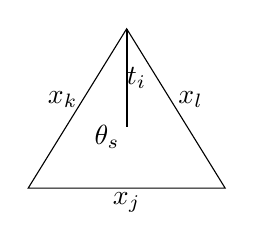
\begin{tikzpicture}[scale=1.25]
 \coordinate (1) at (1,0);
 \coordinate (2) at (-1,0);
 \coordinate (3) at (0,1.618);
 \coordinate (4) at (0, 0.618);
 \draw (1)--(2)--(3)--cycle;
 \draw [thick](3)--(4);
 \node at (-0.2, 0.518) {$\theta_s$};
 \node at (0.1,1.118) {$t_i$};
 \node at (0.65,0.9) {$x_l$};
 \node at (-0.65,0.9) {$x_k$};
 \node at (0,-0.15) {$x_j$};
 \end{tikzpicture}
 \end{center}
 Here, $\theta_s$ is the $\mu$-invariant associated to the face containing $t_i$.
	Finally, we define the weight of a super $T$-path to be the product of the weights of its edges
 \[\wt(t)=\prod_{t_i\in t}\wt(t_i),\]
 where the product of $\mu$-invariants is taken under the positive ordering.
\end{Definition}

 In what follows, we will use $\lambda_{ab}$ to denote the $\lambda$-length of the arc $(a,b)$,
 and we will write $\boxed{ijk}$ to denote the $\mu$-invariant associated to the triple of
 ideal points $(i,j,k)$, subject to Remark~\ref{rem:mu-invariants}.
	
The following theorem is the main result of the current paper, giving an explicit expression for arbitrary super $\lambda$-lengths
in terms of the $\lambda$-lengths and $\mu$-invariants of a fixed triangulation.

\begin{Theorem}\label{thm:main}
Under the default orientation,
 the $\lambda$-length of $(a,b)$ is given by
 \[\lambda_{a,b} = \sum_{t\in\mathcal T_{a,b}} \wt(t).
 \]
\end{Theorem}
